\chapter{Fejlesztői dokumentáció}
\begin{comment}
A Fejlesztői dokumentáció tartalmazza
- a probléma részletes specifikációját,
- a felhasznált módszerek részletes leírását, a használt fogalmak definícióját,
- a program logikai és fizikai szerkezetének leírását (adatszerkezetek, adatbázisok,
modulfelbontás),
- a tesztelési tervet és a tesztelés eredményeit.
\end{comment}

\section{Megoldási terv}
A programot 3 nagy részre lehet bontani: 

\begin{figure}[h]
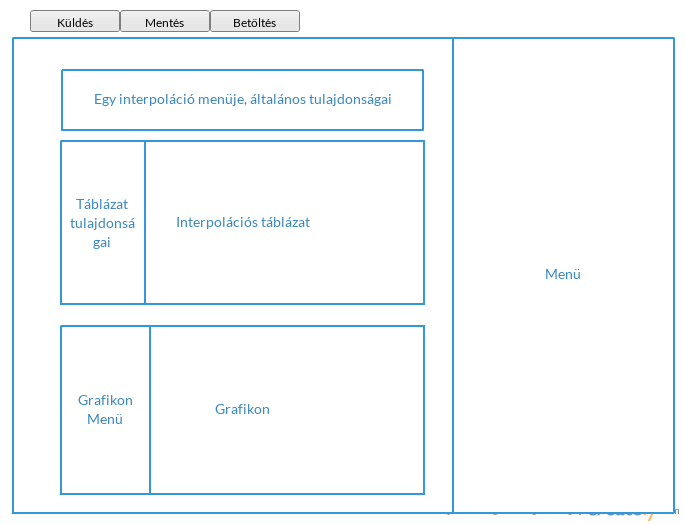
\includegraphics[width=\textwidth]{pics/weblap_vazlat}
\centering
\caption{Weboldal Vázlata}
\end{figure}

\begin{figure}[h]
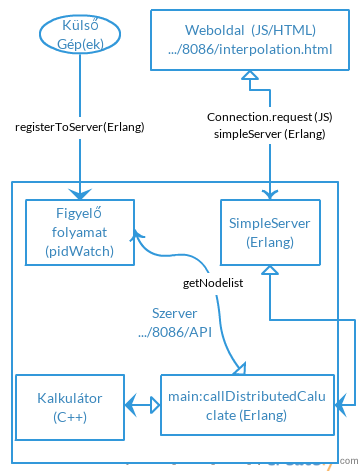
\includegraphics[width=8cm]{pics/kommunikacio}
\centering
\caption{Kommunikáció}
\end{figure}

\section{Weboldal}
Weboldal felépítése HTML és JavaScript segítségével valósult meg. Egy oldalból áll melyen a felhasználó össze állítja a neki szükséges adathalmazt. Új adathalmazokat hozhat létre, a régieket szerkesztheti. A háttérben JSON-be formálódnak az adatok.
Ha a felhasználó végzett egy gombra nyomással a program legenerálja a szükséges objektumot. \newline
A felület sok gombot tartalmaz, melyek hatására frissíthetőek az adatok. Amikor frissítünk egy részt, általában mentődnek az értékek egy inputba JSON formában.\newline
A felület manuálisan lett csak tesztelve, folyamatában ahogyan épült a program.
\subsection{Felépítés}
	A weboldal forráskódja a Webpage mappában helyezkedik el. 
	A fájlszerkezet az alábbi:
	\begin{description}
		\item[webpage.js :] \hfill \\  Globális változók inicializálása és pár alapbeállítás lefuttatása
		\item[webpage.html :]  \hfill \\ Weboldal megjelenítése, fájlok betöltése
		\item[init] 
		\hfill \\ Inicializáló függvények hívásai és események
		\begin{description}
			\item[menulist.js : ]
			\hfill \\ Interpolációk listájának inicializálója
		  	\item[plot.js : ]
		  	\hfill \\ Interpolációs grafikon inicializálása
			\item[table.js : ]
			\hfill \\ Interpolációs táblázat inicializálása
		 	\item[events.js : ]
		 	\hfill \\ Gombra kattintások eseményei
		\end{description}

		\item[model] 
		\hfill \\ Objektumok, melyeket az inicializáló lépésben hívunk, és azok segédletei
		\begin{description}
		 	\item[base.js : ] 
		 		\hfill \\ Globális függvények \newline
		 		Base.get, Base.erlangJSON, Base.forEach
		 	\item[base\_table.js : ] 
		 		\hfill \\
		 		Általános táblázat generáló függvény
		 	\item[connection.js : ] 
		 		\hfill \\Szerver kapcsolat meghívására szolgáló függvény \newline
		 		 Connection.request
		 	\item[plot\_types.js : ]
		 		\hfill \\ A grafikon kirajzoló típus objektumai
		 	\item[polinome.js : ] 
		 		\hfill \\  
		 		Polinóm kirajzolását segítő függvények \newline
		 		makePolinome található benne és egyéb segédfüggvények
		 	\item[web\_page\_debug.js : ] 
		 		\hfill \\ 
		 		A Weboldalon történő logolást segítő objektum
		 		\newline Jelenleg sehol nem használjuk már, de a megvalósítás során fontos szerepe volt a hibajavításban
		\end{description}
		\item[model/interpolation] 
		\hfill \\ Az oldal 3 fő részegységének függvényei
			\begin{description}
			\item[menulist.js : ] Interpolációk lista megvalósítása
			\hfill \\  function interpolationMenulist (aConfig) Objektum fájlja
		  	\item[plot.js : ] Interpolációs grafikon megvalósítása
			\hfill \\  function interpolationPlot(aConfig) Objektum fájlja
			\item[table.js : ] Interpolációs táblázat megvalósítása
			\hfill \\  function interpolationTable(aConfig) Objektum fájlja
			\end{description}
	\end{description}
\subsection{Fontsabb objektumok és függvények}
	\hfill
	Az objetumokat legtöbb esetben egy függvény generálja, melyben that.-al jelöltek azok, melyeket a visszatérés után felhasználunk az eseménykezelésekhez.
	\begin{description}
		\item[makePolinome(inPolinome, plotFor)] 
			\hfill \\ 
			Polinóm pontjainak legenerálására szolgáló függvény, a grafikon kirajzolónak megfelelő típusban
			\begin{description}
			\item[inPolinome] polinóm
			\item[plotFor] polinóm intervalluma és pontossága
			\end{description}
		\item[Connection.request(aConfig)] 
			\hfill \\ 
			Elküldi a szervernek az értékeket
			\begin{description}
			\item[aConfig.params] a kommunikáció objektuma
			\item[aConfig.callback] sikeres visszatérés esetén lefutó függvény
			\end{description}
		\item[basicTable (aConfig)]
			\hfill \\ 
			Egy alap tábla létrehozó objektum. Ennek segítségével tudtam létrehozni az interpolációs táblázatot és a menülistát(interpoláció választó)
			\begin{description}
			\item[that.addNewCellToRow(rowIndex, textValue, inputAttributes)] 
				\hfill \\  Ad egy új cellát a sorhoz
			\item[that.addNewRowToTable(data)]
				\hfill \\ Ad egy új sort a táblázathoz
			\item[that.addNewColumnToTable(data)]
				\hfill \\ Ad egy új oszlopot a táblázathoz
			\item[that.newTable()] 
				\hfill \\ Új tábla létrehozása
			\item[that.setCellForm((i , j, attributes))] 
				\hfill \\ Egy adott cella megformázás beállítása
			\item[that.getNumOfCols()] 
			 	\hfill \\ Vissza adja az oszlopok számát
			\item[that.getNumOfRows()]
				\hfill \\ Vissza adja a sorok számát
			\item[that.getRow(i)]
				\hfill \\ Vissza adja a sort az index alapján. 
				Ha nincs olyan indexű akkor null
			\item[that.getInputTag(i, j)]
				\hfill \\ Vissza tér a tábla input elemével
			\item[that.getValue(i, j)]
				\hfill \\ Egy adott cella érték lekérdezése
			\item[that.findValue(column, value)] 
				\hfill \\ Megkeresi melyik sorban van egy adott értéket
			\item[that.setValue(i, j, value, form)]
				\hfill \\ Beállít egy adott értéket egy cellának
			\item[that.deleteTable()]
				\hfill \\ Teljesen törli a táblázatot
			\item[that.remove(row)]
				\hfill \\ Kivesz egy sort a táblázatból
			\item[addNewRowTagToTable ()]
				\hfill \\ Ad egy új sort a táblázathoz
			\item[addCellToRow(index)]
				\hfill \\ Ad  egy cellát a sorhoz
			\item[setAttributes(object, attributes)]
				\hfill \\ Beállítja egy objektum tulajdonságait
			\item[makeTextInput (value,  attributes)]
				\hfill \\  TextInput hozzáadása a sorhoz
			\end{description}
		\item[interpolationMenulist (aConfig)] 
			\hfill \\ 
			Az interpolációs menü függvénye. Itt tarjuk számon az aktuálisan betöltött adathalmazt.
			\begin{description}
			\item[that.newItem()] 
			\hfill \\ Új Lista elem
			\item[that.getDataArray(server)] 
			\hfill \\ Vissza adja az adathalazt, tömb formában. Ebben a formában küldjük fel a szervernek.
			\item[that.getDataObject()] 
			\hfill \\ Vissza adja az adathalmazt, egy objektum formájában. Az Objektum értékeinek kulcsa, az interpolációk id-ja.
			\item[that.saveItemSettings()] 
			\hfill \\ Elmenti az adatokat az aktuálisan kijelölt sorba.
			\item[that.loadItemSettings(index)]
			\hfill \\ Feldogozza az adatt sort a táblából, és betölti az adatokat a táblába.
			\item[that.loadAll(savedObject, resultObject)] 
			\hfill \\Betölti az összes Interpolációt az adott adathalmazból
			\item[newMenulist()] 
			\hfill \\
			Új menülista: régi menü kitörlése, és egy új generálása
			\hfill \\ 
			\end{description}
		\item[interpolationPlot (aConfig)]
			\hfill \\ Grafikon megjelenítése: Flot segítségével létrehoztam az alábbi Objektumot. Ebben valósítottam meg a kirajzolást, és annak tulajdonságait.
			\begin{description}
			\item[that.refresh(points, polinomials)]
			\hfill \\ Pontok és a polinómok alapján frissíti a grafikont
			\item[that.getPlotSettings]
			\hfill \\ Visszatér a grafikon megjelenítési tulajdonságokkal. Ennek segítségével mentjük el a tulajdonságokat.
			\item[that.setPlotSettings]
			\hfill \\ Betölti a grafikon megjelenítési tulajdonságokat.
			\item[generateData(senderData, polynomial)]
			\hfill \\ Legenrálja a grafikon azon bemenő paraméterét, amely a megjelnítendő adatokat állítja
			\item[generateType()]
			\hfill \\ Legenrálja a grafikon azon bemenő paraméterét, amely a grafikon megjelítését állítja
			\item[setDefaultSettings()]
			\hfill \\ Legenrálja a grafikon azon bemenő paraméterét, amely a grafikon megjelítését állítja
			\item[generatePointSet(tableArray, derivNum)]
			\hfill \\ Legenerálja az adott pontokat, az interpolációs táblázatból
			\end{description}

		\item[interpolationTable (aConfig)]
			\hfill \\ 
				Az interpolációs Táblázat logikája, és generálása. Ebben a táblázatban tekinthetjük meg a pontokat.
			\begin{description}
			\item[that.addPoint(x, y, dn)] 
			\hfill \\ Hozzá adja a pontot a táblázathoz. Ha létetik ezen az X-en pont akkor frissíti.
			\item[that.setPoints(tableArray)] 
			\hfill \\ Feltölti a táblázatot egy adott tömb értékeivel
			\item[that.setData(data)] 
			\hfill \\ Feltölti az adatokkal a táblát
			\item[that.getData()] 
			\hfill \\ Vissza adja a táblázatban szereplő adatok
			\item[that.getPoints()] 
			\hfill \\ Vissza adja a táblázatban szereplő pontokat
			\end{description}
	\end{description}

\section{Elosztott rendszer}
Elosztott rendszer Erlang-ban lett megvalósítva. Az elosztást interpolációnként végezzük, vagyis annyi node-ot hozunk létre amennyi interpolációt kívánunk egyszerre kiszámítani. \newline
A szerver figyel egy portot hogy érkezett-e rá adat. Ha érkezett adat az adott portra, azt kibontja, és elvégzi a szükséges műveleteket. A JSON-t kibontja, és feldolgozza. Kinyer belőle egy listát mely az interpolálni kívánt pontokat és tulajdonságokat tartalmazza. \newline
Tudjuk pontosan hány eleme van a listának, és annyi processz-t hozunk létre. Ha vannak felcsatlakozva Node-ok akkor a processzt az adott node-on is meg tudja hívni.
Ha létrehozta a processzeket lista elemein végig megy, és azokat szétküldi a processzeknek, majd megvárja míg az összes végig ér, és vissza térve megkapja az eredményt.
\subsection{Web-szerver kommunikáció}
\subsubsection{Adat feldolgozás}
	Az adatot JSON-ben kapja a szerver. Az adathalmaz kibontásához MonchiJSON lett alkalmazva.
	Az MochiJSON kibontásához használt segédfügvények:
	\begin{description}
	\item[struct\_handler:getElementByKeyList(KeyList, DataSetElement)]
	\hfill \\ Vissza tér egy értékkel, amely az adott kulcson van, ha egy elemű a kulcs lista. Több elem esetén a kulcsokban lévő értékeket nézi, és vissza adja a legbelső kulcson lévő elemet.
	\item[struct\_handler:getElementByKey()]
	\hfill \\ Vissza tér egy értékkel, amely az adott kulcson van.
	\item[struct\_handler:getElementByKey()]
	\hfill \\ 

	\end{description}

	\begin{description}
	\item[struct\_handler:getDataByJson()]
	\hfill \\ 
	\item[struct\_handler:simplifyPolinomial]
	\hfill \\ Egyszerűsít egy polinómot
	\end{description}
	%% convertToMochi, getPoints, getType, getInverse, getElementByKey simplifyPolinomial getId, getDataSet
\subsection{Gép-szerver kommunikáció}
	\begin{description}
	\item[pidWatch:startPidWatch()]
	\hfill \\ Elindítja a node-figyelőt, melyben feliratkozni lehet a listára, vagy lekérdezni az adatokat. A node-figyelő indulás után figyelni fog és ha küldenek neki egy kérést, akkor azt kezeli. 
	\item[pidWatch:registerToServer(Pong\_Node)]
	\hfill \\ Ezzel a kéréssel lehet felcsatlakozni a szerverre. A kérést elküldi és ha sikeres volt a feliratkozás, akkor ok-al tér vissza.
	\end{description}
\subsection{Elosztás folyamata}
\subsection{Számítás hívása}
	\begin{description}
	\item[calculator:calculateByData(DataSetElement)]
	\hfill \\ A bejövő paraméterből kinyeri a pontokat és a típust, majd meghívja a számító függvényt.
	\item[calculator:calculate(\_X, \_Y, \_Type, \_Inverz)]
	\hfill \\ C++-ban implementált és onnan betöltött függvény
	\end{description}
\subsection{Tesztelési terv}
\subsection{Függvények listája}
	\begin{description}
		\item[]
		\hfill \\ 
	\end{description}

\section{Kalkulátor}
A Kalkulátor részben számítódik ki egy-egy interpolációnak az ereménye.
A megkapott adatok alapján számol, ha kell létre hozza a kezdő mátrixot, kiszámolja az eredmény mátrixot, majd annak segítségével kiszámolja a polinómot.
\subsection{Fontosabb számítási függvények}

\begin{description}
	\item[DArray interpolateMain] 
	\hfill \\ Kívülről meghívandó fő függvény mely elosztja és konvertálja a részeket
	\begin{description}
	  \item[DArray \&x :] Az x pontok listája 
	  \item[DMatrix \&Y :] Az x pontokhoz tartozó y pontok halmaza
	  \item[string type :] Interpóláció típusa: lagrange, newton, hermite
	  \item[bool inverse :] Inverz interpoláció kell-e
	\end{description}
\end{description}
\subsection{Elosztott rendszerrel való kommunikáció}
Az elosztott rendszerben hívódó számítást Erlang - erl\_nif"-el sikerült megoldanom. 
Az ezzel kapcsolatos dolgokat az Calculator/erlang.cpp tartalmazza. 
\subsection{Tesztelési terv}
A tesztelést folyamatosan végeztem a minta adatok alapján. A függvények implementálása közben ezekre a minta adatokra meghívtam, majd ezekkel számoltam. A teszteléshez a logTest.cpp fájlban található függvényeket alkalmaztam. 